\documentclass{SEDESOLab}
\usepackage{ifthen}
% \usepackage[printonlyused,nohyperlinks]{acronym}
\usepackage{acronym}
\usepackage{units}

\usepackage{todonotes}
\usepackage[utf8]{inputenc}
\usepackage{siunitx}
\usepackage{subcaption}

\usepackage{csquotes}
\usepackage{dirtytalk}
\usepackage{supertabular}
\usepackage[section]{placeins}


\newcommand{\img}{./img}
\newcommand{\bib}{./bib}

\newcommand{\e}[1]{\mbox{e}^{#1}}
\graphicspath{{figures/}}



\begin{document}

\colorlet{punct}{red!60!black}
\definecolor{delim}{RGB}{20,105,176}
\colorlet{numb}{magenta!60!black}

\lstdefinelanguage{json}{
    basicstyle=\normalfont\ttfamily,
    numbersep=8pt,
    showstringspaces=false,
    breaklines=true,
    frame=lines,
    literate=
     *{0}{{{\color{numb}0}}}{1}
      {1}{{{\color{numb}1}}}{1}
      {2}{{{\color{numb}2}}}{1}
      {3}{{{\color{numb}3}}}{1}
      {4}{{{\color{numb}4}}}{1}
      {5}{{{\color{numb}5}}}{1}
      {6}{{{\color{numb}6}}}{1}
      {7}{{{\color{numb}7}}}{1}
      {8}{{{\color{numb}8}}}{1}
      {9}{{{\color{numb}9}}}{1}
      {:}{{{\color{punct}{:}}}}{1}
      {,}{{{\color{punct}{,}}}}{1}
      {\{}{{{\color{delim}{\{}}}}{1}
      {\}}{{{\color{delim}{\}}}}}{1}
      {[}{{{\color{delim}{[}}}}{1}
      {]}{{{\color{delim}{]}}}}{1},
  }
%% Enter the deliverable information  in this document (tittle.tex)

%%%%%%%%%%%%%%%%%%%%%%%%%%%%%%%%%%%%%%%%%%%%%%%%%%%%%%%%%%%%%%%%%%%%%%%%%%%%%%%%%%
% First Page
%%%%%%%%%%%%%%%%%%%%%%%%%%%%%%%%%%%%%%%%%%%%%%%%%%%%%%%%%%%%%%%%%%%%%%%%%%%%%%%%%%
\graphicspath{{images/}}

\newcommand{\MyName}{Mónica Zamudio López}
\newcommand{\Institution}{Laboratorio de Datos, SEDESOL}
\newcommand{\DelTitle}{Recolección y limpieza de información}
\newcommand{\DelNumber}{1}
\newcommand{\DelVersion}{0.1/1.0}
\newcommand{\Contrato}{ATN/OC 15822-RG}
\newcommand{\footertext}{\raisebox{3mm}{Entregable \DelNumber}}
\setlength{\footheight}{36pt}
\newcommand{\footerlogo}{\raisebox{3mm}{\leavevmode
\includegraphics[width=2cm]{bid}}}
\clearscrheadfoot
\pagestyle{empty}


% \begin{tikzpicture}[overlay,remember picture]
%   \draw [line width=1pt]
%   ($ (current page.north west) + (1cm,-1cm) $)
%   rectangle
%   ($ (current page.south east) + (-1cm,1cm) $);
% \end{tikzpicture}

\definecolor{SINetblue}{HTML}{07505B}
\newcolumntype{C}{ >{\centering\arraybackslash} m{4cm} }

\begin{center}
SEDESOL 2018
\vspace{0.1cm}

  \begin{center}


  % H2020 has no logo and no visual identity

  % 
\includegraphics[width=0.7\textwidth]{images/LOGO_FJR}
      \Large \MyName \\\vspace{5mm}
\begin{multicols}{2}

\includegraphics[width=0.35\textwidth]{images/bid}

\includegraphics[width=0.25\textwidth]{images/LOGO_FJR}
\end{multicols}
\begin{multicols}{2}

\includegraphics[width=0.4\textwidth]{images/sedesol}

\includegraphics[width=0.2\textwidth]{images/presidencia}
\end{multicols}


  \vspace{2mm}

  \end{center}
  \vspace{0.3cm}
  {\Large Título del proyecto: USO DE DATOS MASIVOS PARA LA EFICIENCIA DEL ESTADO Y LA INTEGRACIÓN REGIONAL\\}
    {\large Clave: \Contrato}\\
  \vspace{0.5cm}
  \Large Puesto: Científico de Datos Junior\\
  \vspace{1.0cm}

  \begin{spacing}{2.5}
    \textbf{\Huge \DelTitle}\\\vspace{10mm}
    \textbf{\Large Entregable número: \DelNumber} \\\vspace{10mm}
  \end{spacing}

  % \vspace*{\fill}

  %just to avoid warning :)
  \newcommand\undefcolumntype[1]{\expandafter\let\csname NC@find@#1\endcsname\relax}
  \newcommand\forcenewcolumntype[1]{\undefcolumntype{#1}\newcolumntype{#1}}
  \forcenewcolumntype{C}{ >{\arraybackslash} m{3cm} }


  % \begin{tabular}{C@{\hspace*{0cm}}l}
  %   % \includegraphics[scale=0.2]{images/logos/EU_Flag_320_213} &
  %   % \begin{tabular}{l}
  %   % {Funded by the European Union’s Horizon 2020 research and innovation programme}\\
  %   % {under the Marie Sklodowska-Curie Grant Agreement No. 699924}\\
  %   \end{tabular}
  % \end{tabular}
\end{center}

\clearpage

%%%%%%%%%%%%%%%%%%%%%%%%%%%%%%%%%%%%%%%%%%%%%%%%%%%%%%%%%%%%%%%%%%%%%%%%%%%%%%%%%%
% Second Page
%%%%%%%%%%%%%%%%%%%%%%%%%%%%%%%%%%%%%%%%%%%%%%%%%%%%%%%%%%%%%%%%%%%%%%%%%%%%%%%%%%
\setlength{\headheight}{0.7cm}
\setlength{\footskip}{18mm}
\addtolength{\textheight}{-\footskip}
\pagestyle{empty}

\begin{flushright}
    \begin{tabular}{lp{11cm}}
    \textbf{Acrónimo del proyecto:}       &   Estimación de Ingreso \\
    \hline
    \textbf{Nombre completo del proyecto:} & USO DE DATOS MASIVOS PARA LA EFICIENCIA DEL ESTADO Y LA INTEGRACIÓN REGIONAL\\
    \hline
    \textbf{Referencia:}                  &   ATN/OC 15822-RG\\
    \hline
%    \textbf{Topic:}                 &   ICT-10-2015 \\
%    \textbf{Type of Action:}        &   RIA \\
    % \textbf{Grant Number:}          &   699924 \\
    \textbf{URL del Proyecto:}           &  \url{http://www.plataformapreventiva.gob.mx}
  \end{tabular}



% define "struts", as suggested by Claudio Beccari in
%    a piece in TeX and TUG News, Vol. 2, 1993.
\newcommand\Tstrut{\rule{0pt}{2.6ex}}         % = `top' strut
\newcommand\Bstrut{\rule[-0.9ex]{0pt}{0pt}}   % = `bottom' strut

  \begin{tabular}{|l|p{115mm}|}\hline
    % \Tstrut\Bstrut Editor:& XXX, XXX-Institution\\\hline
    \Tstrut\Bstrut Tipo de Entregable:& Reporte (R) \\\hline
    % \Tstrut\Bstrut Dissemination level:& Public (PU)\\\hline
    \Tstrut\Bstrut Fecha de Entrega Contractual:& Mayo - 2018\\\hline
    \Tstrut\Bstrut Fecha de Entrega& 3 de Mayo de 2018\\\hline
    % \Tstrut\Bstrut Suggested Readers:&Project partners, future community-lab.net users\\\hline
    \Tstrut\Bstrut Número de Páginas:&\pageref{finalpg}\\\hline
    \Tstrut\Bstrut Keywords:& estimación ingreso ciencia datos ingesta \\\hline
    \Tstrut Autor:&
    \begin{tabular}[t]{l}
      \MyName, \Institution \Bstrut \\
      % XXX - YYY, Institution \\
      % XXX - YYY, Institution \\
      % XXX - YYY, Institution \Bstrut \\
    \end{tabular}\\\hline
  \end{tabular}
\end{flushright}

\section*{Resumen}
La Secretaría de Desarrollo Social (SEDESOL) es una entidad del gobierno mexicano destinada al apoyo de la población para el mejoramiento de sus condiciones de vida.\\
Un problema importante para SEDESOL es la correcta distribución de sus recursos por lo que es importante contar con una metodología que permita la generación de una focalización correcta para así poder ayudar a aquellos que realmente están en condiciones vulnerables.\\
En este reporte se detalla el proceso de obtención e integración de distintas fuentes de información que puedes ser de utilidad en dicho proceso, ya sea de manera directa o como auxiliar de las primeras.\\
Las partes fundamentales para la realización de esto son, el estudio y evaluación de información generada por la misma Secretaría como lo es el Cuestionario Único de Información Socioeconómica (CUIS) y el Sistema de Focalización de Desarrollo (SIFODE), además de datos auxiliares que permitan la georreferenciación como archivos poligonales de carreteras y caminos. Para esto es importante llevar a cabo un sistema semiautomatizado para almacenar de manera adecuada todas las fuentes de datos para su futuro uso así como la información de los orígenes y naturaleza de las mismas.
\clearpage






% \oddsidemargin=5mm
% \evensidemargin=5mm
% \textwidth=30cm

% \topmargin=0cm
% \textheight=40\baselineskip
\setcounter{tocdepth}{2}

\tableofcontents

%% SHOULD be included if the deliverable becomes large
% \input{executivesummary}

%% COMMANDS
%%
%% \acresetall	flushes the ’memory’ of the macro \ac (ie all "used" marks flushed)
%%
%% \ac{label}	singular (first time Full Name + (ACRO) and mark as used)
%% \acp{label}	plural (as \ac but makes short and/or long forms into plurals)
%%
%% \acs{lable}	short (ACRO)
%% \acf{lable}	“full acronym” (Full Name + (ACRO))
%% \acl{lable}	long (_without_ ACRO)
%%
%% \acsp{label}	short plural (ACROs)
%% \acfp{label}	“full acronym” plural (Full Names + (ACROs))
%% \aclp{label}	long plural (_without_ ACRO)
%%
%% \acrodef{label}[acronym]{written out form}	definition
%%		for example \acrodef{etacar}[$\eta$ Car]{Eta Carinae},
%%		with the restriction that the label should be simple ASCII


%% PACKAGE & OPTIONS
%% acronym package must be loaded (in the preamble):
%%    \usepackage[option1,option2,etc.]{acronym}
%% OPTIONS:
%%    footnote		The option footnote makes the full name appear as a
%%			footnote.
%%    nohyperlinks	If hyperref is loaded, all acronyms will link to their
%%			glossary entry. With the option nohyperlinks these
%%			linkscan be suppressed.
%%    printonlyused	Only list used acronyms
%%    withpage		In printonlyused-mode show the page number where
%%			each acronym was first used.
%%    smaller		Make the acronym appear smaller.
%%    dua			The option dua stands for “don’t use acronyms”. It
%%			leads to a redefinition of \ac and \acp, making the
%%			full name appear all the time and suppressing all
%%			acronyms but the explicity requested by \acf or \acfp.
%%    nolist		The option nolist stands for “don’t write the list of
%%			acronyms”.


%% INCLUSION
%%
\chapter*{Lista de Acrónimos}
\label{sec:acronimos}

\begin{acronym}[ENIGH] %width of the longest acronym should be matched here
    \acro{DGGPB}{Dirección General de Geoestadística y Padrones de Beneficiarios}
    \acro{DGAE}{Dirección General Adjunta de Análisis Espacial}
    \acro{DGAIP}{Dirección General Adjunta de Integración de Padrones}
  \acro{CUIS}{Cuestionario Único de Información Socioeconómica}
  \acro{SIFODE}{Sistema de Focalización de Desarrollo}
  \acro{SEDESOL}{Secretaría de Desarrollo Social}
  \acro{ENIGH}{Encuesta Nacional de Ingresos y Gastos de los Hogares}
  \acro{PEA}{Población Económicamente Activa}
  \acro{LGDS}{Ley General de Desarrollo Social}
  \acro{INEGI}{Instituto Nacional de Estadística y Geografía}
  \acro{SISI}{Sistema de Información Social Integral}
  \acro{PUB}{Padrón Universal de Beneficiarios}
  \acro{AWS}{Amazon Web Services}

\end{acronym}
\clearpage


% ------------------------
% Chapter
% ------------------------

\clearscrheadfoot

% uncomment for book mode
%\lofoot{\footerlogo}
%\refoot{\footerlogo}
%\lefoot{\footertext}
%\rofoot{\footertext}

%\rohead{\pagemark}
%\lohead{\DelTitle}
%\lehead{\pagemark}
%\rehead{\DelTitle}

%\cfoot[\pagemark]{}

\lofoot[\footerlogo \hspace{10pt} \footertext]{\footerlogo \hspace{10pt} \footertext}
\lefoot[\footerlogo \hspace{10pt} \footertext]{\footerlogo \hspace{10pt} \footertext}

\refoot[\pagemark]{\pagemark}
\rofoot[\pagemark]{\pagemark}

\rohead{\rightmark}
\rehead{\rightmark}

\lohead{\leftmark}
\lehead{\leftmark}




\setcounter{page}{1}
\pagestyle{scrheadings}

\chapter{Introducción}
\section{Sección Uno}

\section{Sección Dos}

\chapter{Consideraciones finales para ajustar el modelo}
\label{chap:ajuste}
\section*{El modelo: recapitulación y avances}
\subsection*{Fuentes de datos}
Como se mencionó en \cite{mzl_entregable_2}, la fuente principal de datos para el ajuste del modelo fue la Encuesta de Características Socioeconómicas de los Hogares, o ENCASEH. Esta encuesta contiene los módulos definidos en el CUIS como base, y puede ser complementada con módulos adicionales de preguntas que se consideren necesarias para la focalización, según el objetivo del programa en cuestión. Para nosotros fue de particular interés utilizar los datos de PROSPERA, que incluyen el módulo de verificaciones domiciliarias. Así, podemos considerar el problema de reportaje incorrecto como un problema de datos faltantes según el marco de análisis planteado por \cite{missing_data}, utilizando el módulo de verificaciones domiciliarias como etiquetas\footnote{Aquí queda implícito el primer supuesto importante que hacemos en la modelación: que no hay error en las verificaciones. Es decir, que las variables verificadas siempre reflejan las verdaderas características de los hogares.}. La idea del enfoque de datos faltantes es entonces explotar la distribución conjunta entre las respuestas a los cuestionarios y las variables verificadas para poder imputar datos dado un conjunto de evidencia.
\par
\noindent
\\
Ahora, es plausible pensar que la distribución de las características de los hogares cambie conforme nos encontremos en municipios con distintos perfiles de carencias o marginación. Eso nos llevó a incluir una segunda fuente de en el modelo: los datos de marginación a nivel municipal, publicados por el CONAPO. Estos datos consisten en un índice de marginación, que es esencialmente la primera componente resultante de aplicar el método de componentes principales a este conjunto de variables\footnote{Todas las variables se miden en porcentaje de la población que satisface la característica mencionada.}:
\begin{itemize}
    \item Población de 15 años o más analfabeta
    \item Población de 15 años o más sin primaria terminada
    \item Viviendas particulares habitadas sin drenaje ni servicio sanitario
    \item Viviendas particulares habitadas sin energía eléctrica
    \item Viviendas particulares habitadas sin agua entubada
    \item Viviendas particulares habitadas con piso de tierra
    \item Viviendas particulares habitadas con algún nivel de hacinamiento
    \item Población en localidades con menos de cinco mil habitantes
    \item Población ocupada con ingreso de hasta dos salarios mínimos
\end{itemize}
Dado que los levantamientos contienen referencias al domicilio en el que se encuentra la vivienda, podemos utilizar esa información para filtrar en tiempo real los valores correspondientes al municipio que contiene a ese domicilio. Sin embargo, utilizar dos conjuntos distintos de variables (el conjunto con las variables a nivel municipio y el conjunto original) añade ciertas dificultades para la comparación entre modelos, de las que hablaremos más adelante.
\subsection*{El proceso de modelado}
Recordemos que estamos ajustando una red bayesiana a los datos. Una red bayesiana en un grupo de variables $V = (X_1, X_2, \dots, X_n)$ es una gráfica dirigida G, con $V$ como su conjunto de vértices. La gráfica $G$ representa las distribuciones cuya conjunta se puede escribir como $p(x_1, x_2, \dots, x_n) = \prod_{i=1}^{n}p(x_i|pa(x_i))$, donde $pa(x_i)$ es el conjunto de variables que son padres de $x_i$ en la gráfica $G$.
\par
\noindent
Notemos cómo esta definición induce una propiedad de Markov en la red bayesiana: los nodos representan variables aleatorias y las aristas relaciones de probabilidad, por lo que la estructura de la red define una factorización de la función de distribución conjunta en un conjunto de distribuciones \textit{locales} de probabilidad, una para cada variable\footnote{Para más detalle sobre esto, ver \cite{bayesian_networks}.}. Debido a la correspondencia entre independencia condicional y separación gráfica, es posible aprender primero la estructura de la gráfica, y dada una estructura, estimar las distribuciones locales una por una, sin las complicaciones inducidas por la dimensionalidad de los datos.
\section*{El método}
Independientemente del algoritmo que se escoja para encontrar la estructura de la gráfica, el método convencional para ajustar una red bayesiana a un conjunto de datos es el siguiente:
\begin{enumerate}
    \item Aprender la estructura de la gráfica a través de un algoritmo apropiado.
    \item Estimar los parámetros de las distribuciones locales para cada nodo, utilizando una distribución multinomial para variables categóricas y una distribución normal multivariada para variables continuas\footnote{En este caso, los modelos son mayormente conocidos como Redes Bayesianas \textit{Gaussianas}, y las variables aleatorias se relacionan entre sí a partir de restricciones lineales.}
\end{enumerate}
\subsection*{El algoritmo}
Para ajustar la red bayesiana en R, escogimos el paquete \texttt{bnlearn}: un paquete que incluye distintos tipos de algoritmos para el aprendizaje de la estructura, con un conjunto bastante grande de métricas de evaluación a escoger.
\par
\noindent
Los algoritmos que aprenden la estructura de una gráfica se dividen en dos grandes categorías: basados en restricciones y basados en puntuación (constraint-based y score-based, respectivamente). Hasta ahora, no existe evidencia concluyente que apunte a la superioridad de algún tipo sobre el otro (ver \cite{algorithm_comparison}), por lo que decidimos utilizar \texttt{hill climbing}: un algoritmo \textit{greedy} basado en puntuación que pertenece a la familia de algoritmos de búsqueda local.
\subsection*{Parámetros relevantes}
Por su naturaleza, el algoritmo permite especificar ciertos parámetros de búsqueda que pueden ser optimizados para obtener mejores resultados:
\begin{itemize}
    \item \textbf{blacklist/whitelist}: conjunto de aristas a excluir/incluir del modelo. En cualquiera de los dos casos, especificar este conjunto permite que el algoritmo descarte estructuras irrelevantes. En nuestro caso, descartamos todas las aristas de variables reportadas a variables verificadas, y también todas las aristas hacia variables a nivel municipal que no partieran de otra variable a nivel municipal.
    \item \textbf{score}: la medida de ''bondad de ajuste'' a ser utilizada para la evaluación de las posibles estructuras. Existen muchas medidas posibles de evaluación, pero todas tienen que asignar el mismo puntaje a las estructuras que tengan asociada la misma distribución de probabilidad conjunta. En este caso, se utilizó siempre el AIC, o Criterio de Información de Akaike.
    \item \textbf{restarts}: número de ''recomienzos'' que hace el algoritmo para evitar caer en un mínimo local.
    \item \textbf{k}: coeficiente de penalización por el número de parámetros estimados. Es importante incluir algún grado de penalización para prevenir el sobreajuste.
\end{itemize}

\chapter{Evaluación del modelo}
\label{chap:evaluacion}
Recordemos que el problema que buscamos resolver a través de este modelo es el de priorizar correctamente las verificaciones domiciliarias, reduciendo así la proporción de hogares que son sujetos a un proceso de focalización incorrecta. Dada la deriva temporal a la que está sujeto el proceso de focalización -los programas que operan en cierta región, así como los criterios que utilizan para focalizar, están cambiando constantemente- simplificamos el problema al definir que nuestro objetivo es, simplemente, asignar correctamente las verificaciones. Definimos como una verificación correctamente asignada a aquella en la que se tuvo que corregir el valor de al menos una variable. Así, podemos utilizar la distribución posterior resultante de nuestro modelo bayesiano para definir un clasificador que indique una verificación a realizar en caso de que haya una probabilidad de tener cambios suficientemente alta.
\par
\noindent
Podemos entonces comparar entre conjuntos de variables como comparamos entre clasificadores. Sin embargo, dado un conjunto de variables, necesitamos escoger el valor de $k$ que resulte en la estructura más adecuada. Definimos entonces nuestro proceso de evaluación de modelos en dos pasos.
\section*{Comparación de estructuras}
Lo primero que necesitamos asegurar es que, dado un conjunto de variables, tenemos la mejor estructura posible que el algoritmo sea capaz de encontrar. Necesitamos escoger entonces una medida de bondad de ajuste para la distribución conjunta inducida por la estructura de la gráfica.
\par
\noindent
Dado que escogimos un modelo bayesiano, resulta natural pensar en la verosimilitud -o alguna transformación monótona de esa función- para evaluar modelos. En nuestro caso, decidimos utilizar la devianza de prueba por la facilidad de interpretarla de forma análoga a la suma de cuadrados residuales, en el caso de regresión lineal por mínimos cuadrados\footnote{Es decir, que una devianza de validación en el modelo "perfecto" o saturado es igual a cero, y la devianza de validación incrementa conforme el ajuste del modelo empeora}. La devianza de prueba para un modelo $M_0$, que estima $\hat{\mu} := E[Y|\hat{\theta}_0]$ basada en las observaciones $y$ está definida por:
\begin{align*}
D(y, \hat{\mu}) &= 2(log(p(y|\hat{\theta}_s)) - log(p(y|\hat{\theta}_0)))
\end{align*}
Donde $\hat{\theta}_0$ denota los valores de los parámetros del modelo a evaluar $M_0$, y $\hat{\theta}_s$ denota los valores de los parámetros del modelo \textbf{saturado}. Esta métrica nos permite, dado un conjunto de variables, escoger el valor de $k$ que nos dé la mejor estructura posible para minimizar la devianza.
\par
\noindent
Después de un poco de exploración con las restricciones, decidimos considerar los siguientes seis modelos:
\begin{enumerate}
\item \textbf{Modelo sin restricciones}: modelo que incluye solamente las variables reportadas y verificadas, sin ninguna restricción para el algoritmo de búsqueda de estructura.
\item \textbf{Modelo base}: modelo que incluye solamente las variables reportadas y verificadas, con la restricción de que no exista una arista de una variable reportada a una verificada.
\item \textbf{Modelo base + variables municipales}: modelo base con las variables a nivel municipal que componen el índice de marginación de CONAPO.
\item \textbf{Modelo base + GM}: modelo base con la variable de grado de marginación: una discretización del índice de marginación a través del método Dalenius.
\item \textbf{Modelo base + variables municipales + GM}: modelo base con la variable de grado de marginación y con todas las variables municipales que lo componen.
\item \textbf{Modelo base + 3 variables municipales}: modelo base con tres variables a nivel municipal: analfabetismo, falta de drenaje/excusado y hacinamiento.
\end{enumerate}
Para efectos analíticos, discretizamos todas las variables a nivel municipal con estas tres categorías:$(0-10, 11-40, 41-100)$. La estructura resultante en cada modelo se encuentra adjunta en el anexo.
\par
\noindent
Utilizando la métrica propuesta, comparamos cada uno de los modelos para escoger el mejor valor del parámetro de regularización. Los resultados preliminares son los siguientes:
\begin{figure}[h]
    \caption{Devianza de validación para todos los modelos considerados.\\
    \textit{Dado que la razón de verosimilitud tiene un denominador distinto (estamos considerando distintos conjuntos de variables), no es comparable entre gráficas.}}
    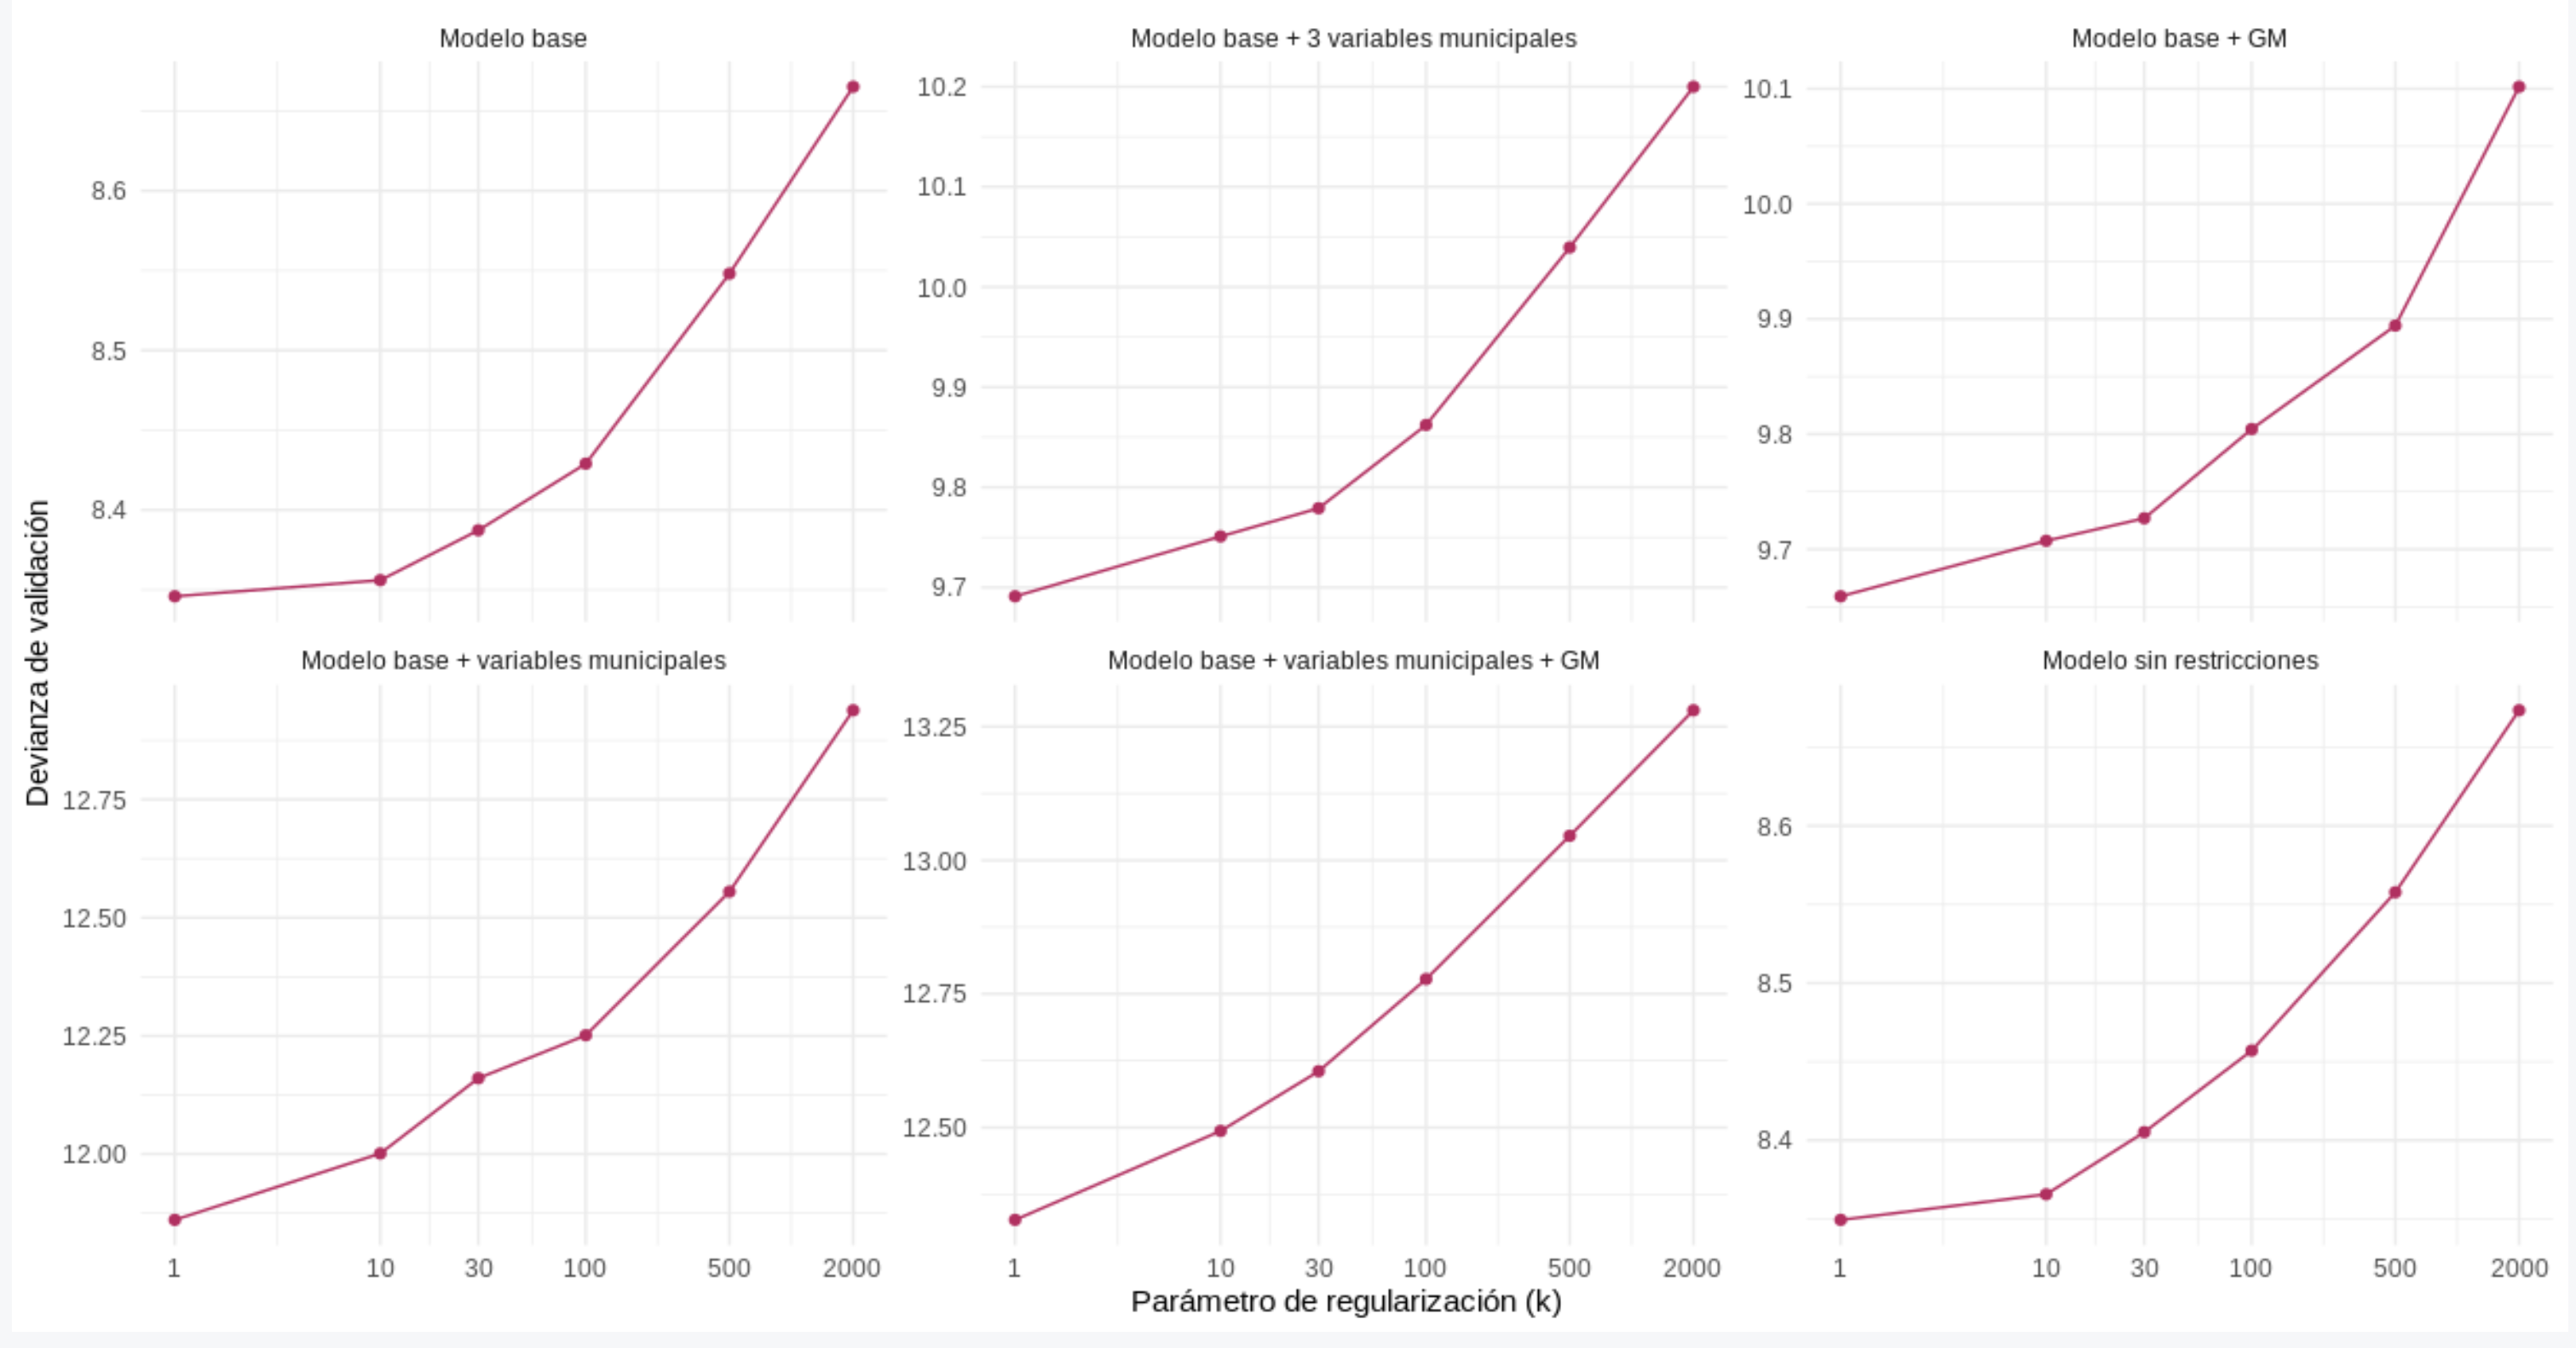
\includegraphics[height=14cm, width=18cm]{devianza_validacion}
\end{figure}
\section*{Comparando distintos conjuntos de variables}
Una vez que escogimos la mejor estructura posible dado un conjunto de variables, es necesario construir el clasificador que mencionamos anteriormente. Necesitamos entonces hacer inferencia probabilística para obtener un estadístico que nos ayude con la tarea de clasificación.
\par
\noindent
Existen varios algoritmos para hacer inferencia en Redes Bayesianas. Nosotros consideramos dos: \textit{logic sampling} -parte de la familia de técnicas de muestreo por importancia- y \textit{belief propagation}, un algoritmo de paso de mensaje. La ventaja del segundo sobre el primero es que permite el cálculo de las distribuciones marginales de manera más eficiente. Además, las técnicas de muestreo por importancia pueden llevar a descartar buena parte de los elementos de la muestra, resultando así en un tiempo mayor de convergencia. Sin embargo, los algoritmos de muestreo por importancia que están implementados en R tienen menos carga de dependencias, lo cual puede resultar útil en la implementación como explicaremos más adelante.\\
Una vez que calculamos la distribución posterior de las variables ''verdaderas'' dadas las respuestas al cuestionario, podemos hacer una comparación simple y construir un estadístico que podamos interpretar como la probabilidad de tener algún incorrecto. Para esto, lo que hicimos fue restar las probabilidades de las respuestas (codificadas como variables binarias) y sumar esas diferencias. En la siguiente figura podemos observar la distribución de este estadístico, según el verdadero estado de reportaje en el cuestionario.
\begin{figure}[H]
    \caption{Suma de probabilidades según la distribución a posteriori}
    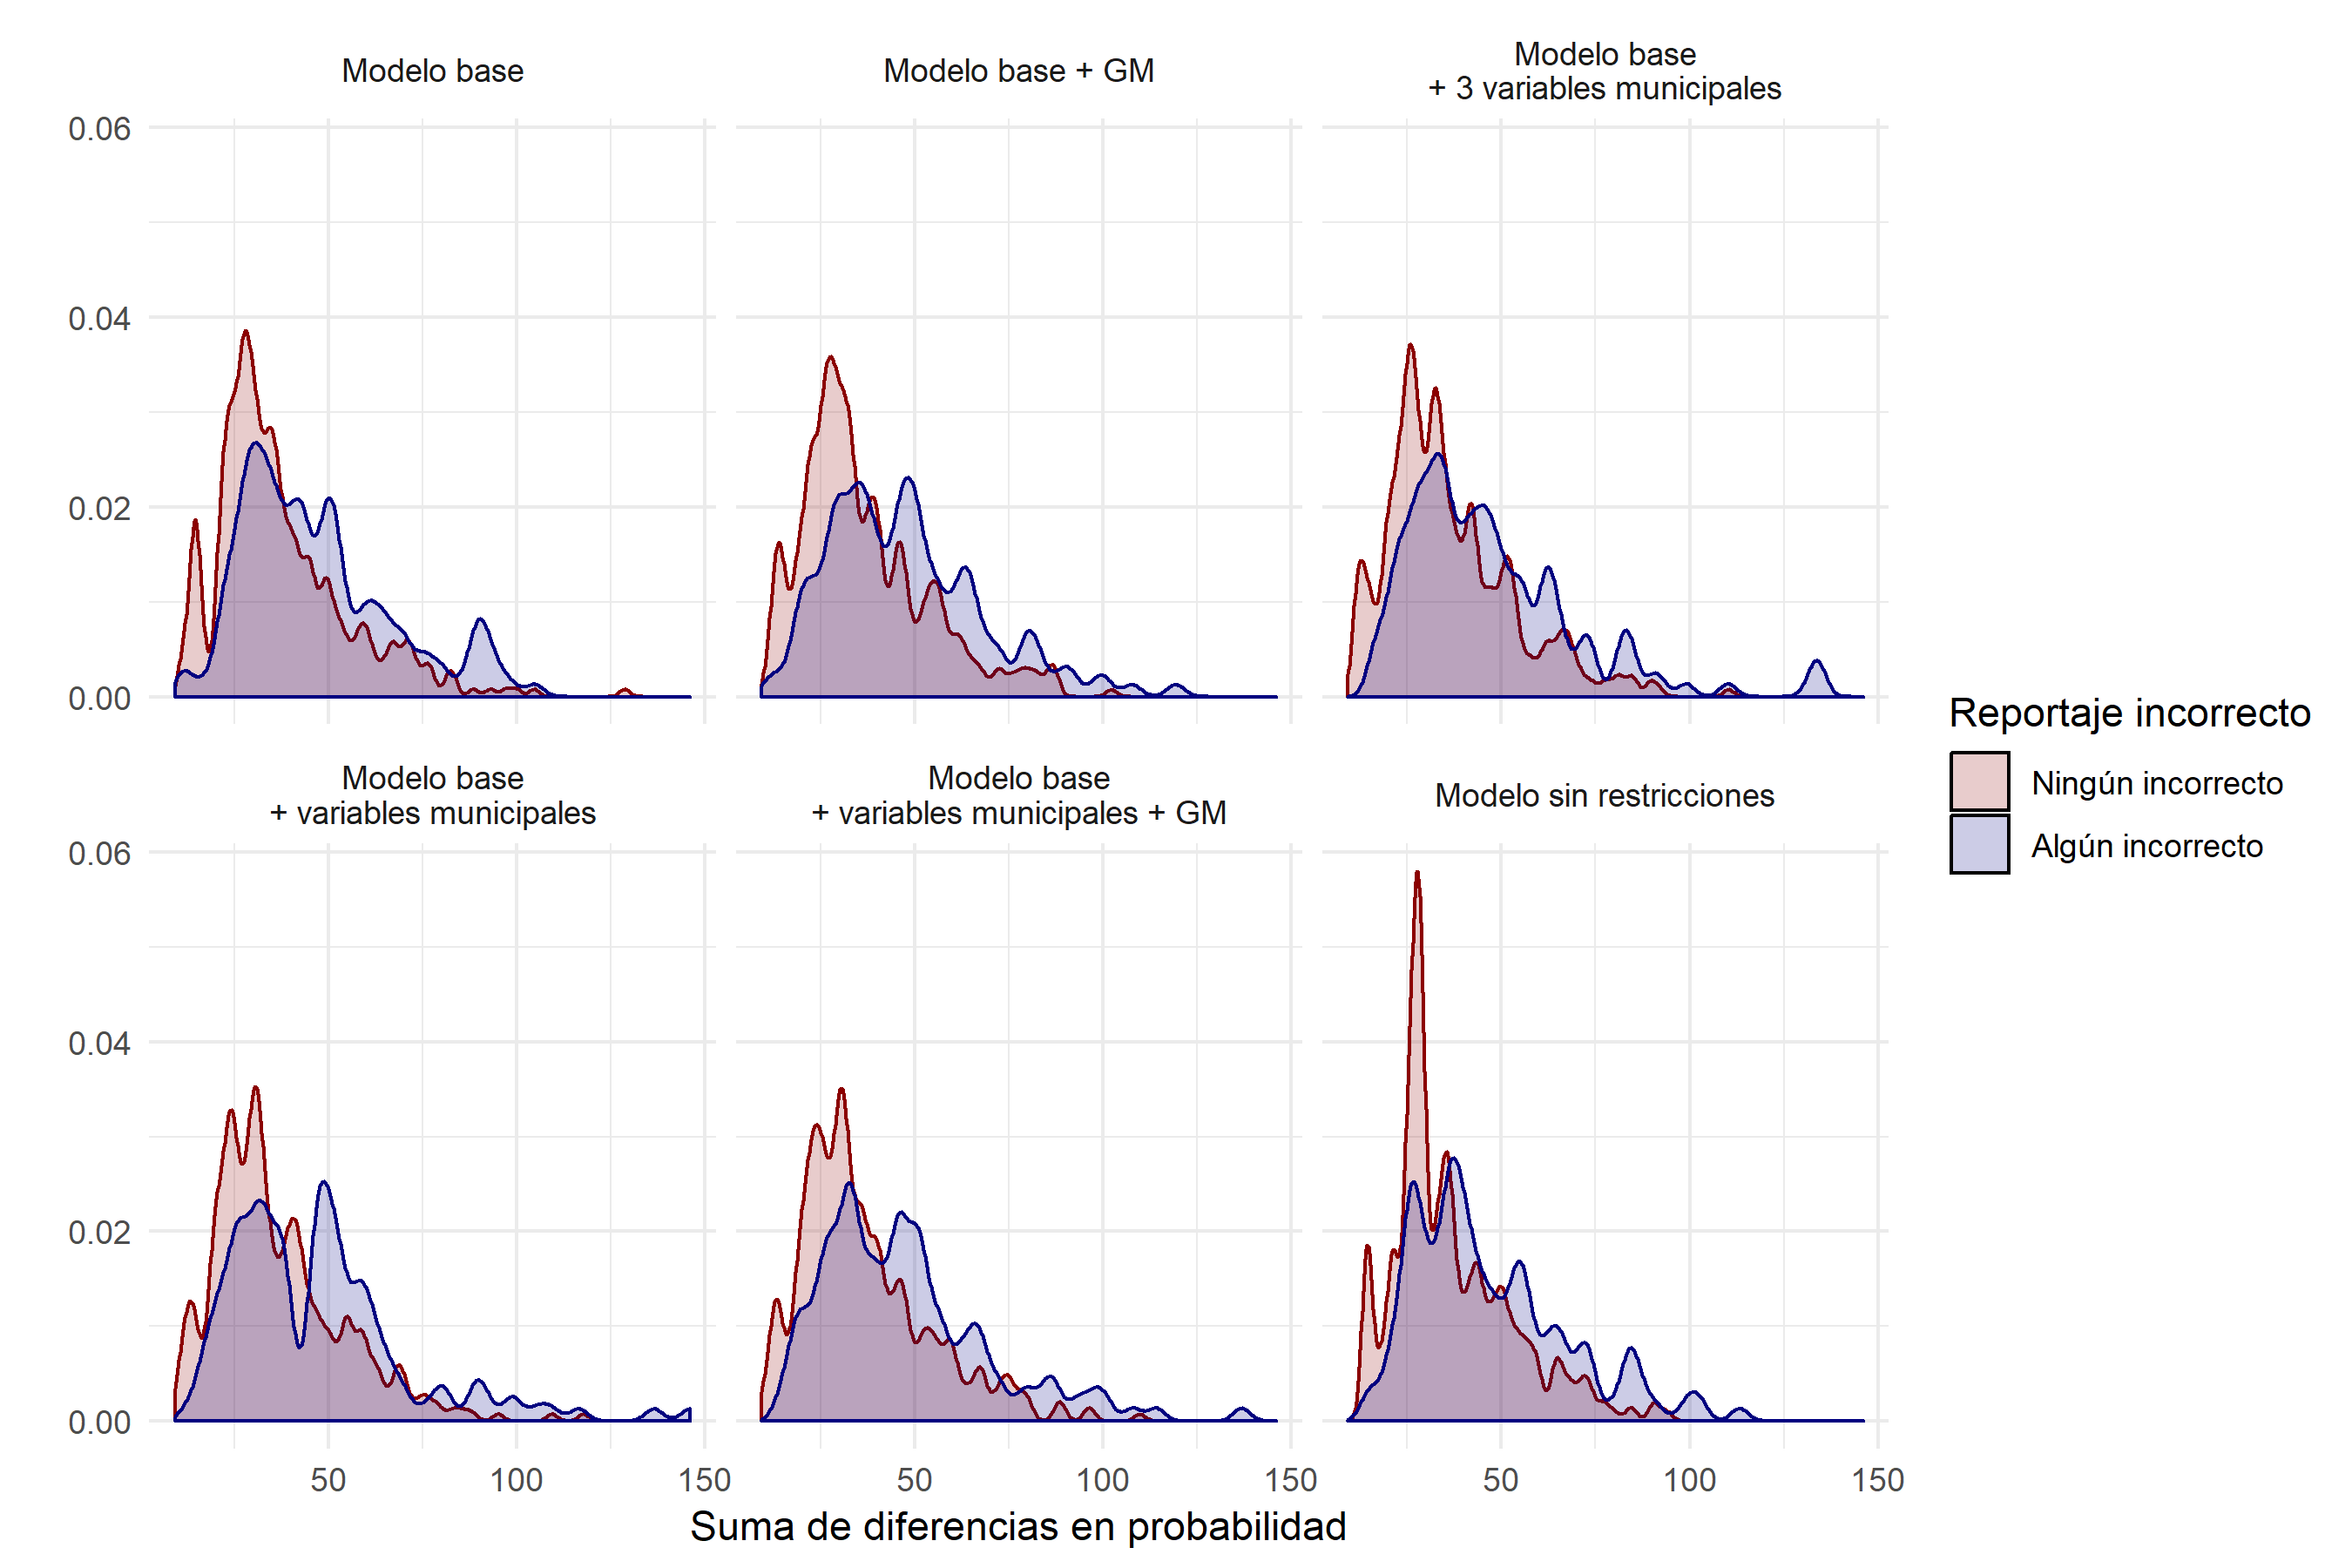
\includegraphics[width=18cm, height=12cm]{suma_probabilidades}
    {\footnotesize{Comparando las distribuciones que induce cada modelo, notemos que si bien las que tienen algún error están más sesgadas a la derecha, en general no parece fácil establecer las diferencias entre estas y las distribuciones sin error. Esto implica que necesitamos explorar más opciones para construir un mejor clasificador.}}
\end{figure}
\par
\noindent
Una vez obtenida la suma, comparamos varios puntos de corte para construir un clasificador binario, y evaluamos el clasificador utilizando el área bajo la curva ROC. La curva ROC (Receiver Operating Characteristic, por su origen naval) es una herramienta para evaluar la capacidad de un clasificador binario de discriminar conforme va variando el umbral de clasificación. Esta curva resulta de graficar la Tasa de Falsos Positivos (TFP) en el eje x, y la tasa de verdaderos positivos (TVP) en el eje Y. Estas dos métricas se definen como sigue:
\begin{align*}
    TFP := \frac{FP}{N} \\
    TVP := \frac{VP}{P}
\end{align*}
Donde $(F,V)$ son Falso y Verdadero, y $(N,P)$ son Negativo y Positivo, respectivamente. Cabe mencionar que a la TVP comúnmente se le llama \textit{sensitividad}, y que la TFP puede reescribirse como $1-TVN$, donde $TVN$ también es conocida como \textit{especificidad}. Ambas métricas son relativamente estándar en el campo de la ciencia de datos, y compararlas gráficamente tiene la intención de tomar en cuenta el intercambio que se hace entre falsos positivos y falsos negativos en la construcción de un clasificador.
\par
\noindent
\begin{figure}[H]
    \caption{Curva ROC}
    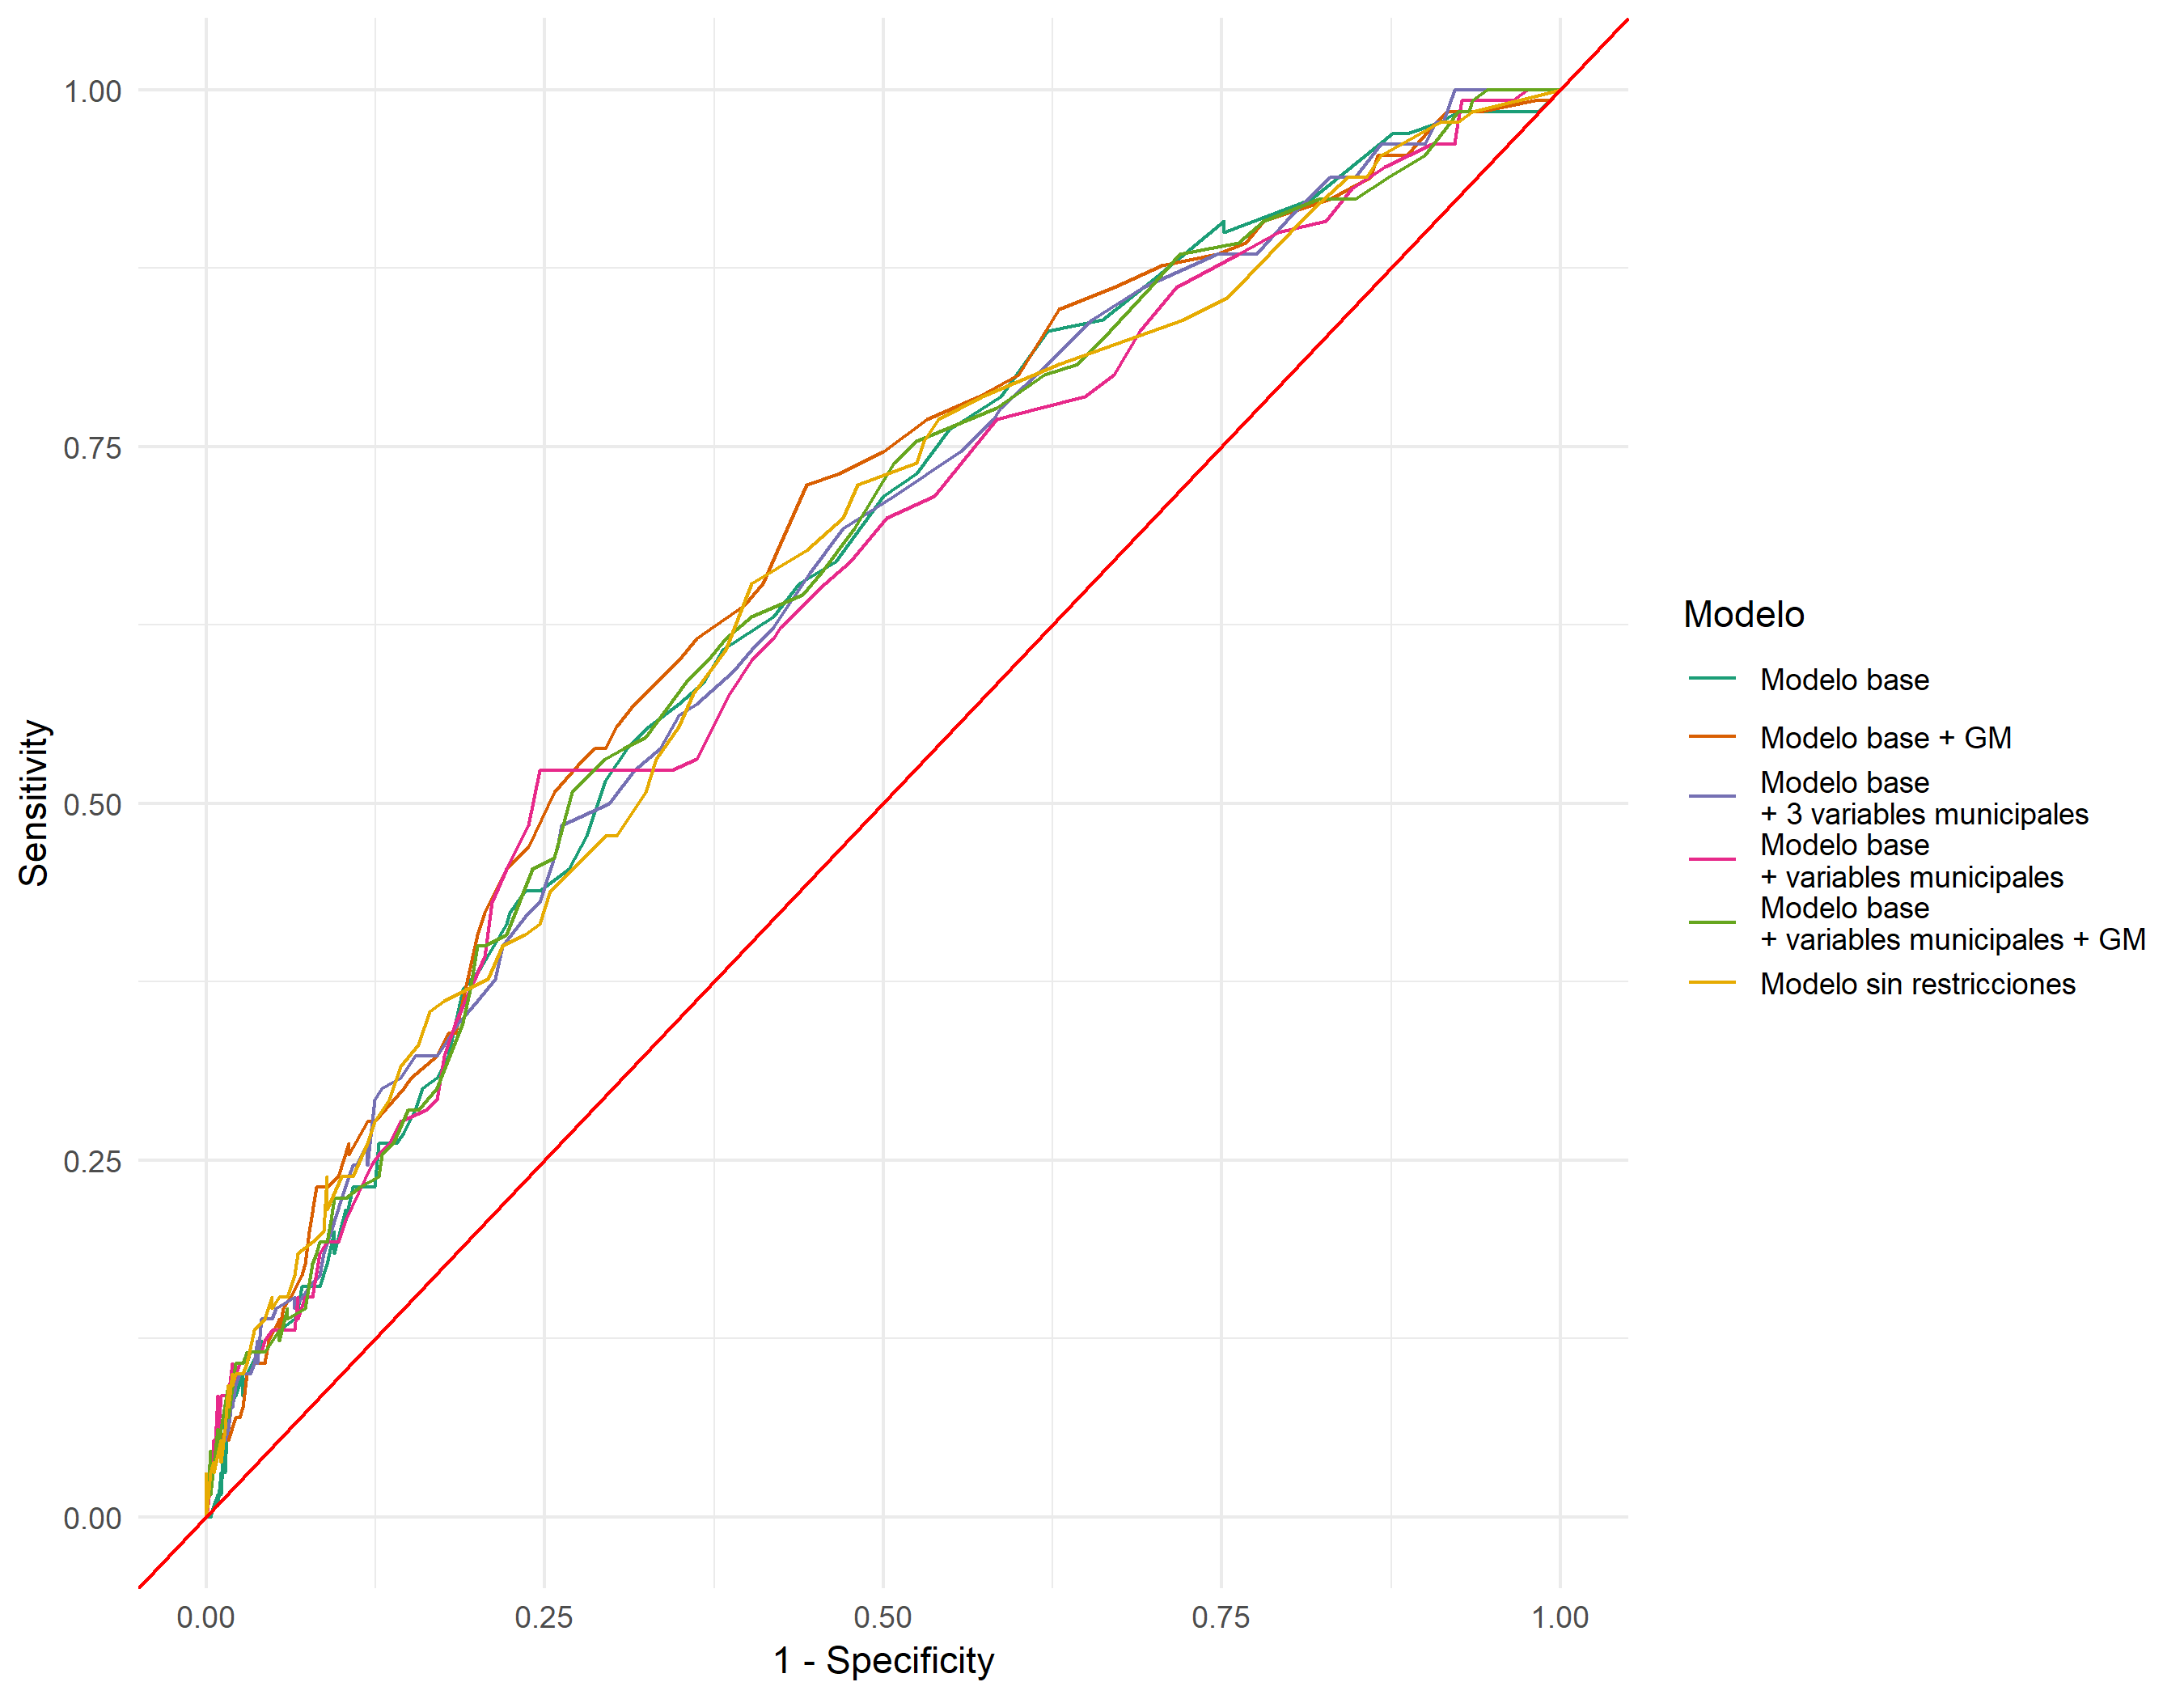
\includegraphics[height=14cm, width=18cm]{results_roc}
\end{figure}
Intuitivamente, la curva ROC de un clasificador perfecto sería una $L$ reflejada sobre el eje horizontal, y la curva ROC de un clasificador construido tirando una moneda sería la línea roja $y=x$.
\par
\noindent
Ahora, para poder evaluar la efectividad general de cada clasificador, tomando en cuenta todos los puntos de corte, se utiliza generalmente el área bajo la curva ROC (AUC, por sus siglas en inglés). En este caso utilizamos la Regla del Trapecio para calcular el AUC a partir de la colección de puntos obtenida.
\begin{figure}[H]
    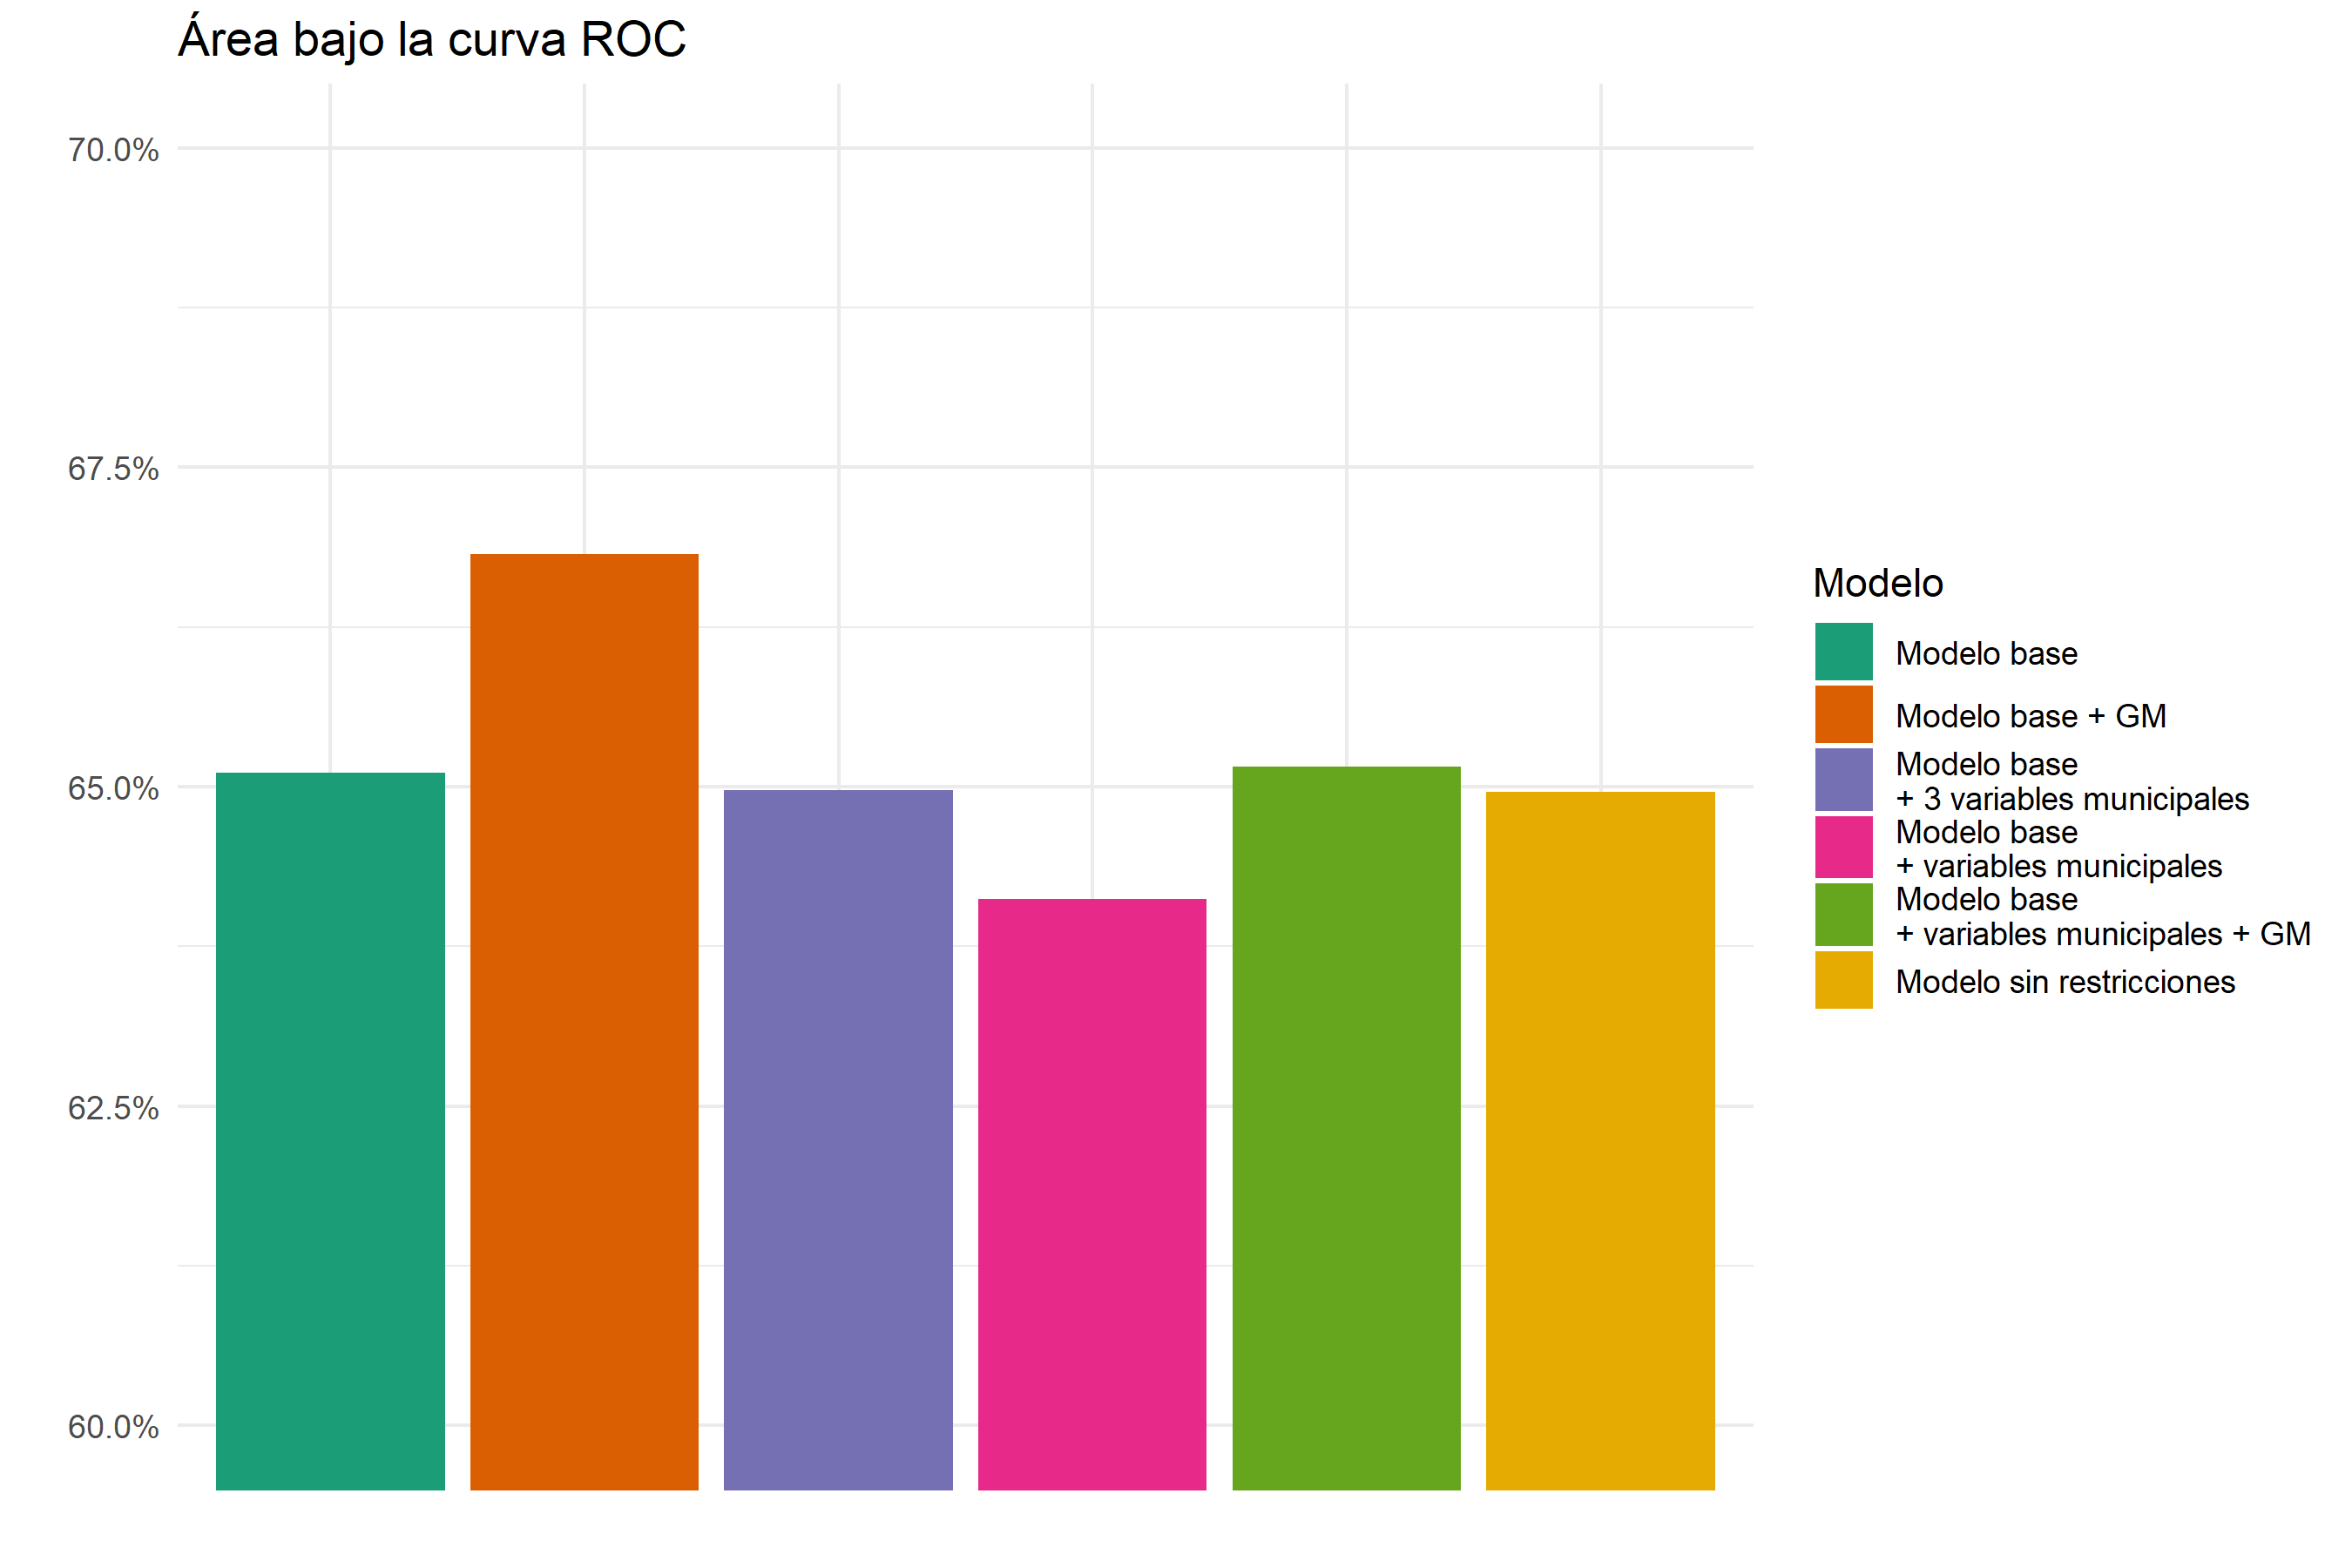
\includegraphics[height=14cm, width=18cm]{results_auc}
    \footnotesize{Notemos que hemos limitado el rango del eje y para efectos de comparabilidad entre modelos, pero el resultado del AUC varía relativamente poco entre ellos.}
\end{figure}
Los resultados indican que el Modelo Base con grado de marginación induce un clasificador ligeramente mejor que los otros. Además, si comparamos las estructuras de los modelos, el grado de marginación sí parece estar resumiendo gran parte de la información que tienen el resto de las variables. Decidimos utilizar este modelo para la implementación del piloto, pero tenemos una serie de recomendaciones para seguir esta exploración:
\begin{itemize}
    \item Explorar más conjuntos de variables a nivel municipal, y otro tipo de discretizaciones.
    \item Reentrenar el modelo con los resultados del piloto. Intuitivamente, tiene sentido pensar que las tasas de reportaje incorrecto sean mayores en programas que no hacen verificaciones domiciliarias a todos sus cuestionarios.
    \item Explorar los patrones de sub y sobrerreporte obtenidos del piloto, buscando reducir la dimensionalidad del problema.
\end{itemize}


\bibliography{bib/references}
\appendix
\chapter{Apéndice}
\lstinputlisting[language=bash,basicstyle=\ttfamily\scriptsize,caption={Archivo de ingesta de Red Carretera}]{code/red_carretera.sh}
\pagebreak
\lstinputlisting[language=bash,basicstyle=\ttfamily\scriptsize,caption={Archivo de ingesta de Sifode Calificación}]{code/sifode_calificacion.sh}
\pagebreak
\lstinputlisting[language=bash,basicstyle=\ttfamily\scriptsize,caption={Archivo de ingesta de Sifode Domicilio}]{code/sifode_domicilio.sh}
\pagebreak
\lstinputlisting[language=python,basicstyle=\ttfamily\scriptsize,caption={Archivo de ingesta de Sifode}]{code/sifode.py}
\pagebreak
\lstinputlisting[language=json,basicstyle=\ttfamily\scriptsize,caption={Catálogo},breaklines=true]{code/catalog.json}

\label{finalpg}
\clearpage

\thispagestyle{empty}
\begin{center}
% \vfill
% \begin{figure}
% \centering
% \vspace{3cm}
  % 
\includegraphics[width=10cm]{images/LOGO_FJR}

\begin{multicols}{2}

\includegraphics[width=0.35\textwidth]{images/bid}

\includegraphics[width=0.25\textwidth]{images/LOGO_FJR}
\end{multicols}
\begin{multicols}{2}

\includegraphics[width=0.4\textwidth]{images/sedesol}

\includegraphics[width=0.2\textwidth]{images/presidencia}
\end{multicols}

% \end{figure}
% \vfill
{\large USO DE DATOS MASIVOS PARA LA EFICIENCIA DEL ESTADO Y LA INTEGRACIÓN REGIONAL\\[0.5cm] }
{\large \today \\[0.5cm] }
{\large FJR-\DelNumber-\Contrato\\[0.5cm] }
\vfill

SEDESOL 2018

\doclicenseLicense
\end{center}


%\printbibliography
\end{document}
